%\documentclass[ number=5
			   ,series=sidl
			   ,isbn=xxx-x-xxxxxx-xx-x
			   ,url=http://langsci-press.org/catalog/book/17
			   ,output=long   % long|short|inprep              
			   %,blackandwhite
			   %,smallfont
			   ,draftmode   
			  ]{LSP/langsci}                          

\usepackage{LSP/lsp-styles/lsp-gb4e}		% verhindert Komma bei mehrfachen Fußnoten?
                                                      
\usepackage{layout}
\usepackage{lipsum}

%%%% ABOVE FOR LangSciPress %%%%
%%%% ABOVE FOR LangSciPress %%%%
%%%% ABOVE FOR LangSciPress %%%%
\usepackage{libertine}%work-around solution for rendering problematic characters ʦ, ͡  (mostly in \textbf{})

\usepackage{longtable}%Double-lines (\hline\hline) aren’t typeset properly in ‘longtable’-environment across several pages! conflict with other package (maybe xcolor with option ‘tables’?)

\usepackage{multirow}

\usepackage{array} %allows, among other things, centering column content in a table while also specifying width, creates new column style "x" for center-alignment, "y" for right-alignment
\newcolumntype{x}[1]{>{\centering\hspace{0pt}}p{#1}}%
\newcolumntype{y}[1]{>{\raggedleft\hspace{0pt}}p{#1}}%

\usepackage[]{placeins}%using \FloatBarrier command, all floats still floating at that point will be typeset, and cannot cross that boundary. the option here \usepackage[section]{placeins} automatically adds \FloatBarrier to every \section command (only works for \section commands, nothing lower than that!)
%\usepackage{afterpage}%by using the command \afterpage{\clearpage}, all floats will appear, but no new page will be started, thus avoiding bad page breaks around floats

\usepackage{vowel} %for vowel space chart


%%%IS THIS NECESSARY??
%%%%following allows you to refer to footnotes (from http://anthony.liekens.net/index.php/LaTeX/MultipleFootnoteReferences)
%\newcommand{\footnoteremember}[2]{
%  \footnote{#2}
%  \newcounter{#1}
%  \setcounter{#1}{\value{footnote}}
%} \newcommand{\footnoterecall}[1]{
%  \footnotemark[\value{#1}]} 
%%%%previous allows you to refer to footnotes: use \footnoteremember{referenceText} in footnote, then \footnoterecall{referenceText} to refer.

\usepackage{tikz}%
\usetikzlibrary{plothandlers,matrix,decorations.text,shapes.arrows,shadows,chains,positioning,scopes}

\usepackage{synttree} %zeichnet linguistische Bäume
\branchheight{36pt}%sets height between rows in synttree

\usepackage{lscape}%used for landscape pages in index (list of recordings)

\usepackage{polyglossia}
\setmainlanguage{english}


%%%TAKE OUT FOR FINAL VERSION:
%%%TAKE OUT FOR FINAL VERSION:
%%%TAKE OUT FOR FINAL VERSION:

%%%%following readjusts margin text!
%\setlength{\marginparwidth}{20mm}
%\let\oldmarginpar\marginpar
%\renewcommand\marginpar[1]{\-\oldmarginpar[\raggedleft\footnotesize\vspace{-7pt}\color{red}\It{→ #1}]%
%{\raggedright\footnotesize\vspace{-7pt}\color{red}\It{→ #1}}}
%%%%previous readjusts margin text!

%%%The following lines set depth of ToC (LSP default is only 3 levels)!
%%%\renewcommand{\contentsname}{Table of Contents} % überschrift des inhaltsverzeichnisses
%\setcounter{secnumdepth}{5}%sets how deep section/subsection/subsubsections are numbered
%\setcounter{tocdepth}{5}%sets the depth of the ToC %but this doesn't seem to work!!!
%% new commands for LSP book (Grammar of Pite Saami, by J. Wilbur)

\newcommand{\PS}{Pite Saami}
\newcommand{\PSDP}{Pite Saami Documentation Project}
\newcommand{\WLP}{Wordlist Project}

\newcommand{\HANG}{\everypar{\hangindent15pt \hangafter1}}%also useful for table cells
\newcommand{\FB}{\FloatBarrier}%shortcut for this command to print all floats w/o pagebreak

\newcommand{\REF}[1]{(\ref{#1})}%adds parenthesis around the reference number, particularly useful for examples.%\Ref had clash with LSP!
\newcommand{\dline}{\hline\hline}%makes a double line in a table
\newcommand{\superS}[1]{\textsuperscript{#1}}%adds superscript element
\newcommand{\sub}[1]{$_{#1}$}%adds subscript element
\newcommand{\Sc}[1]{\textsc{#1}}%shortcut for small capitals (not to be confused with \sc, which changes the font from that point on)
\newcommand{\It}[1]{\textit{#1}}%shortcut for italics (not to be confused with \it, which changes the font from that point on)
\newcommand{\Bf}[1]{\textbf{#1}}%shortcut for bold (not to be confused with \bf, which changes the font from that point on)
\newcommand{\BfIt}[1]{\textbf{\textit{#1}}}
\newcommand{\BfSc}[1]{\textbf{\textsc{#1}}}
\newcommand{\Tn}[1]{\textnormal{#1}}%shortcut for normal text (undo italics, bolt, etc.)
\newcommand{\MC}{\multicolumn}%shortcut for multicolumn command in tabular environment - only replaces command, not variables!
\newcommand{\MR}{\multirow}%shortcut for multicolumn command in tabular environment - only replaces command, not variables!
\newcommand{\TILDE}{∼}%U+223C %OLD:~}%shortcut for tilde%command ‘\Tilde’ clashes with LSP!%
\newcommand{\BS}{\textbackslash}%backslash
\newcommand{\Red}[1]{{\color{red}{#1}}}%for red text
\newcommand{\Blue}[1]{{\color{blue}{#1}}}%for blue text
\newcommand{\PLUS}{+}%nicer looking plus symbol
\newcommand{\MINUS}{-}%nicer looking plus symbol
%    Was die Pfeile betrifft, kannst Du mal \Rightarrow \mapsto \textrightarrow probieren und dann \mathbf \boldsymbol oder \pbm dazutun.
\newcommand{\ARROW}{\textrightarrow}%→%dieser dicke Pfeil ➜ wird nicht von der LSP-Font unterstützt: %\newcommand{\ARROW}{{\fontspec{DejaVu Sans}➜}}
\newcommand{\DARROW}{\textleftrightarrow}%↔︎%DoubleARROW
\newcommand{\BULLET}{•}%
%%✓ does not exist in the default LSP font!
\newcommand{\CH}{\checkmark}%%\newcommand{\CH}{\fontspec{Arial Unicode MS}✓}%CH as in CHeck
%%following used to separate alternation forms for consonant gradation and umlaut patterns:
\newcommand{\Div}{‑}%↔︎⬌⟷⬄⟺⇔%non-breaking hyphen: ‑  
\newcommand{\QUES}{\textsuperscript{?}}%marks questionable/uncertain forms

\newcommand{\jvh}{\mbox{\It{j}-suffix} vowel harmony}%
%\newcommand{\Ptcl}{\Sc{ptcl} }%just shortcut for glossing ‘particle’
%\newcommand{\ATTR}{{\Sc{attributive}}}%shortcut for ATTRIBUTIVE in small caps
%\newcommand{\PRED}{{\Sc{predicative}}}%shortcut for PREDICATIVE in small caps
%\newcommand{\COMP}{{\Sc{comparative}}}%shortcut for COMPARATIVE in small caps
%\newcommand{\SUPERL}{{\Sc{superlative}}}%shortcut for SUPERLATIVE in small caps
\newcommand{\SG}{{\Sc{singular}}}%shortcut for SINGULAR in small caps
\newcommand{\DU}{{\Sc{dual}}}%shortcut for DUAL in small caps
\newcommand{\PL}{{\Sc{plural}}}%shortcut for PLURAL in small caps
%\newcommand{\NOM}{{\Sc{nominative}}}%shortcut for NOMINATIVE in small caps
%\newcommand{\ACC}{{\Sc{accusative}}}%shortcut for ACCUSATIVE in small caps
%\newcommand{\GEN}{{\Sc{genitive}}}%shortcut for GENITIVE in small caps
%\newcommand{\ILL}{{\Sc{illative}}}%shortcut for ILLATIVE in small caps
%\newcommand{\INESS}{{\Sc{inessive}}}%shortcut for INESSIVE in small caps
\newcommand{\ELAT}{{\Sc{elative}}}%shortcut for ELATIVE in small caps
%\newcommand{\COM}{{\Sc{comitative}}}%shortcut for COMITATIVE in small caps
%\newcommand{\ABESS}{{\Sc{abessive}}}%shortcut for ABESSIVE in small caps
%\newcommand{\ESS}{{\Sc{essive}}}%shortcut for ESSIVE in small caps
%\newcommand{\DIM}{{\Sc{diminutive}}}%shortcut for DIMINUTIVE in small caps
%\newcommand{\ORD}{{\Sc{ordinal}}}%shortcut for ORDINAL in small caps
%\newcommand{\CARD}{{\Sc{cardinal}}}%shortcut for CARDINAL in small caps
%\newcommand{\PROX}{{\Sc{proximal}}}%shortcut for PROXIMAL in small caps
%\newcommand{\DIST}{{\Sc{distal}}}%shortcut for DISTAL in small caps
%\newcommand{\RMT}{{\Sc{remote}}}%shortcut for REMOTE in small caps
%\newcommand{\REFL}{{\Sc{reflexive}}}%shortcut for REFLEXIVE in small caps
%\newcommand{\PRS}{{\Sc{present}}}%shortcut for PRESENT in small caps
%\newcommand{\PST}{{\Sc{past}}}%shortcut for PAST in small caps
%\newcommand{\IMP}{{\Sc{imperative}}}%shortcut for IMPERATIVE in small caps
%\newcommand{\POT}{{\Sc{potential}}}%shortcut for POTENTIAL in small caps
\newcommand{\PROG}{{\Sc{progressive}}}%shortcut for PROGRESSIVE in small caps
\newcommand{\PRF}{{\Sc{perfect}}}%shortcut for PERFECT in small caps
\newcommand{\INF}{{\Sc{infinitive}}}%shortcut for INFINITIVE in small caps
%\newcommand{\NEG}{{\Sc{negative}}}%shortcut for NEGATIVE in small caps
\newcommand{\CONNEG}{{\Sc{connegative}}}%shortcut for CONNEGATIVE in small caps
\newcommand{\ATTRs}{{\Sc{attr}}}%shortcut for ATTR in small caps
\newcommand{\PREDs}{{\Sc{pred}}}%shortcut for PRED in small caps
%\newcommand{\COMPs}{{\Sc{comp}}}%shortcut for COMP in small caps
%\newcommand{\SUPERLs}{{\Sc{superl}}}%shortcut for SUPERL in small caps
\newcommand{\SGs}{{\Sc{sg}}}%shortcut for SG in small caps
\newcommand{\DUs}{{\Sc{du}}}%shortcut for DU in small caps
\newcommand{\PLs}{{\Sc{pl}}}%shortcut for PL in small caps
\newcommand{\NOMs}{{\Sc{nom}}}%shortcut for NOM in small caps
\newcommand{\ACCs}{{\Sc{acc}}}%shortcut for ACC in small caps
\newcommand{\GENs}{{\Sc{gen}}}%shortcut for GEN in small caps
\newcommand{\ILLs}{{\Sc{ill}}}%shortcut for ILL in small caps
\newcommand{\INESSs}{{\Sc{iness}}}%shortcut for INESS in small caps
\newcommand{\ELATs}{{\Sc{elat}}}%shortcut for ELAT in small caps
\newcommand{\COMs}{{\Sc{com}}}%shortcut for COM in small caps
\newcommand{\ABESSs}{{\Sc{abess}}}%shortcut for ABESS in small caps
\newcommand{\ESSs}{{\Sc{ess}}}%shortcut for ESS in small caps
%\newcommand{\DIMs}{{\Sc{dim}}}%shortcut for DIM in small caps
%\newcommand{\ORDs}{{\Sc{ord}}}%shortcut for ORD in small caps
%\newcommand{\CARDs}{{\Sc{card}}}%shortcut for CARD in small caps
\newcommand{\PROXs}{{\Sc{prox}}}%shortcut for PROX in small caps
\newcommand{\DISTs}{{\Sc{dist}}}%shortcut for DIST in small caps
\newcommand{\RMTs}{{\Sc{rmt}}}%shortcut for RMT in small caps
\newcommand{\REFLs}{{\Sc{refl}}}%shortcut for REFL in small caps
\newcommand{\PRSs}{{\Sc{prs}}}%shortcut for PRS in small caps
\newcommand{\PSTs}{{\Sc{pst}}}%shortcut for PST in small caps
\newcommand{\IMPs}{{\Sc{imp}}}%shortcut for IMP in small caps
\newcommand{\POTs}{{\Sc{pot}}}%shortcut for POT in small caps
\newcommand{\PROGs}{{\Sc{prog}}}%shortcut for PROG in small caps
\newcommand{\PRFs}{{\Sc{prf}}}%shortcut for PRF in small caps
\newcommand{\INFs}{{\Sc{inf}}}%shortcut for INF in small caps
\newcommand{\NEGs}{{\Sc{neg}}}%shortcut for NEG in small caps
\newcommand{\CONNEGs}{{\Sc{conneg}}}%shortcut for CONNEG in small caps

\newcommand{\subNP}{{\footnotesize\sub{NP}}}%shortcut for NP (nominal phrase) in subscript
\newcommand{\subVC}{{\footnotesize\sub{VC}}}%shortcut for VC (verb complex) in subscript
\newcommand{\subAP}{{\footnotesize\sub{AP}}}%shortcut for NP (adjectival phrase) in subscript
\newcommand{\subAdvP}{{\footnotesize\sub{AdvP}}}%shortcut for AdvP (adverbial phrase) in subscript
\newcommand{\subPP}{{\footnotesize\sub{PP}}}%shortcut for NP (postpoistional phrase) in subscript

\newcommand{\ipa}[1]{{\fontspec{Linux Libertine}#1}}%specifying font for IPA characters

\newcommand{\SEC}{§}%standardize section symbol and spacing afterwards
%\newcommand{\SEC}{§\,}%

\newcommand{\Nth}{{\footnotesize(\It{n})}}%used in table of numerals in ADJ chapter

%%newcommands for tables in introductionSDL.tex:
\newcommand{\cliticExs}[3]{\Tn{\begin{tabular}{p{28mm} c p{28mm} p{35mm}}\It{#1}&\ARROW &\It{#2} & ‘#3’\\\end{tabular}}}%specifically for the two clitic examples
\newcommand{\Grapheme}[1]{\It{#1}}%formatting for graphemes in orthography tables
%%new command for the section on orthographic examples; syntax: #1=orthography, #2=phonology, #3=gloss
\newcommand{\SpellEx}[3]{\Tn{\begin{tabular}{p{70pt} p{70pt} l}\ipa{/#2/}&\It{#1}& ‘#3’ \\\end{tabular}}}%formatting for orthographic examples (intro-Chapter)


%%new transl tier in gb4e; syntax: #1=free translation (in single quotes), #2=additional comments, z.B. literal meaning:
\newcommand{\Transl}[2]{\trans\Tn{‘#1’ #2}}%new transl tier in gb4e;
\newcommand{\TranslMulti}[2]{\trans\hspace{12pt}\Tn{‘#1’ #2}}%new transl tier in gb4e for a dialog to be included under a single example number


%% used for examples in the Prosody and Segmental phonology chapters:
\newcommand{\PhonGloss}[7]{%PhonGloss = Phonology Gloss;
%pattern: \PhonGloss{label}{phonemic}{phonetic}{orthographic}{gloss}{recording}{utterance}
\ea\label{#1}
\Tn{\begin{tabular}[t]{p{30mm} l}
\ipa{/#2/}	& \It{#4} \\
\ipa{[#3]}	&\HANG ‘#5’\\%no table row can start with square brackets! thus the workaround with \MC
\end{tabular}\hfill\hyperlink{#6}{{\small\textnormal[pit#6#7]}}%\index{Z\Red{rec}!\Red{pit#6}}\index{Z\Red{utt}!\Red{pit#6#7} \Blue{Phon}}
}
\z}
\newcommand{\PhonGlossWL}[6]{%PhonGloss = Phonology Gloss for words from WORDLIST, not from corpus!;
%pattern: \PhonGloss{label}{phonemic}{phonetic}{orthographic}{gloss}{wordListNumber}
\ea\label{#1}
\Tn{\begin{tabular}[t]{p{30mm} l}
\ipa{/#2/}	& \It{#4} \\
\ipa{[#3]}	&\HANG ‘#5’\\%no table row can start with square brackets! thus the workaround with \MC
\end{tabular}\hfill\hyperlink{explExs}{{\small\textnormal[#6]}}%\index{Z\Red{wl}!\Red{#6}\Blue{Phon}}
}
\z}

%%for derivation examples in the derivational morphology chapter!
%syntax: \DerivExam{#1}{#2}{#3}{#4}{#5}{#6}
%#1: base, #2: base-gloss, #3: derived form, #4: derived form gloss, #5: derived form translation, #6: pit-recording, #7: utterance number
\newcommand{\DW}{28mm}%for following three commands, to align arrows throughout
%%%%OLD:
%%%\newcommand{\DerivExam}[7]{\Tn{\begin{tabular}[t]{p{\DW}cl}\It{#1}&\ARROW&\It{#3}\\#2&&#4\\\end{tabular}\hfill\pbox{.3\textwidth}{\hfill‘#5’\\\hbox{}\hfill\hyperlink{pit#6}{{\small\textnormal[pit#6.#7]}}}
%%%%\index{Z\Red{rec}!\Red{pit#6}}\index{Z\Red{utt}!\Red{pit#6.#7}}
%%%}}
%NEW:
\newcommand{\DerivExam}[7]{\Tn{
\begin{tabular}[t]{p{\DW}x{5mm}l}\It{#1}&\ARROW&\It{#3}\\\end{tabular}\hfill‘#5’\\
\hspace{1mm}\begin{tabular}[t]{p{\DW}x{5mm}l}#2&&#4\\\end{tabular}\hfill\hyperlink{pit#6}{{\small\textnormal[pit#6.#7]}}
%\index{Z\Red{rec}!\Red{pit#6}}\index{Z\Red{utt}!\Red{pit#6.#7}}
}}
%%same as above, but supress any reference to a specific utterance
\newcommand{\DerivExamX}[7]{\Tn{
\begin{tabular}[t]{p{\DW}x{5mm}l}\It{#1}&\ARROW&\It{#3}\\\end{tabular}\hfill‘#5’\\
\hspace{1mm}\begin{tabular}[t]{p{\DW}x{5mm}l}#2&&#4\\\end{tabular}\hfill\hyperlink{pit#6}{{\small\textnormal[pit#6]\It{e}}}
%\index{Z\Red{rec}!\Red{pit#6}}\index{Z\Red{utt}!\Red{pit#6.#7}}
}}
\newcommand{\DerivExamWL}[6]{\Tn{
\begin{tabular}[t]{p{\DW}x{5mm}l}\It{#1}&\ARROW&\It{#3}\\\end{tabular}\hfill‘#5’\\
\hspace{1mm}\begin{tabular}[t]{p{\DW}x{5mm}l}#2&&#4\\\end{tabular}\hfill\hyperlink{explExs}{{\small\textnormal[#6]}}
%\index{Z\Red{wl}!\Red{#6}}
}}


%formatting of corpus source information (after \transl in gb4e-environments):
\newcommand{\Corpus}[2]{\hspace*{1pt}\hfill{\small\mbox{\hyperlink{pit#1}{\Tn{[pit#1.#2]}}}}%\index{Z\Red{rec}!\Red{pit#1}}\index{Z\Red{utt}!\Red{pit#1.#2}}
}%
\newcommand{\CorpusE}[2]{\hspace*{1pt}\hfill{\small\mbox{\hyperlink{pit#1}{\Tn{[pit#1.#2]}}\It{e}}}%\index{Z\Red{rec}!\Red{pit#1}}\index{Z\Red{utt}!\Red{pit#1.#2}\Blue{-E}}
}%
%%as above, but necessary for recording names which include an underline because the first variable in \href understands _ but the second variable requires \_
\newcommand{\CorpusLink}[3]{\hspace*{1pt}\hfill{\small\mbox{\hyperlink{pit#1}{\Tn{[pit#2.#3]}}}}%\index{Z\Red{rec}!\Red{pit#2}}\index{Z\Red{utt}!\Red{pit#2.#3}}
}%
%%as above, but for newer recordings which begin with sje20 instead of pit
\newcommand{\CorpusSJE}[2]{\hspace*{1pt}\hfill{\small\mbox{\hyperlink{sje20#1}{\Tn{[sje20#1.#2]}}}}%\index{Z\Red{rec}!\Red{sje20#1}}\index{Z\Red{utt}!\Red{sje20#1.#2}}
}%
\newcommand{\CorpusSJEE}[2]{\hspace*{1pt}\hfill{\small\mbox{\hyperlink{sje20#1}{\Tn{[sje20#1.#2]}}\It{e}}}%\index{Z\Red{rec}!\Red{sje20#1}}\index{Z\Red{utt}!\Red{sje20#1.#2}\Blue{-E}}
}%











%%hyphenation points for line breaks
%%add to TeX file before \begin{document} with:
%%%%hyphenation points for line breaks
%%add to TeX file before \begin{document} with:
%%%%hyphenation points for line breaks
%%add to TeX file before \begin{document} with:
%%\include{hyphenationSDL}
\hyphenation{
ab-es-sive
affri-ca-te
affri-ca-tes
Ahka-javv-re
al-ve-o-lar
com-ple-ments
%check this:
de-cad-es
fri-ca-tive
fri-ca-tives
gemi-nate
gemi-nates
gra-pheme
gra-phemes
ho-mo-pho-nous
ho-mor-ga-nic
mor-pho-syn-tac-tic
or-tho-gra-phic
pho-neme
pho-ne-mes
phra-ses
post-po-si-tion
post-po-si-tion-al
pre-as-pi-ra-te
pre-as-pi-ra-ted
pre-as-pi-ra-tion
seg-ment
un-voiced
wor-king-ver-sion
}
\hyphenation{
ab-es-sive
affri-ca-te
affri-ca-tes
Ahka-javv-re
al-ve-o-lar
com-ple-ments
%check this:
de-cad-es
fri-ca-tive
fri-ca-tives
gemi-nate
gemi-nates
gra-pheme
gra-phemes
ho-mo-pho-nous
ho-mor-ga-nic
mor-pho-syn-tac-tic
or-tho-gra-phic
pho-neme
pho-ne-mes
phra-ses
post-po-si-tion
post-po-si-tion-al
pre-as-pi-ra-te
pre-as-pi-ra-ted
pre-as-pi-ra-tion
seg-ment
un-voiced
wor-king-ver-sion
}
\hyphenation{
ab-es-sive
affri-ca-te
affri-ca-tes
Ahka-javv-re
al-ve-o-lar
com-ple-ments
%check this:
de-cad-es
fri-ca-tive
fri-ca-tives
gemi-nate
gemi-nates
gra-pheme
gra-phemes
ho-mo-pho-nous
ho-mor-ga-nic
mor-pho-syn-tac-tic
or-tho-gra-phic
pho-neme
pho-ne-mes
phra-ses
post-po-si-tion
post-po-si-tion-al
pre-as-pi-ra-te
pre-as-pi-ra-ted
pre-as-pi-ra-tion
seg-ment
un-voiced
wor-king-ver-sion
}\begin{document}\tableofcontents\clearpage

%%%%%%%%%%%%%%%%%%%%%%%%%%%%%%%% ALL THE ABOVE TO BE COMMENTED OUT FOR COMPLETE DOCUMENT! %%%%%%%%%%%


\chapter{Introduction}\label{introChapter}%

This description of the grammar of the \PS\ language is intended to provide a general linguistics audience with an overview of phonological and morphosyntactic structures found in the language. It is based on a corpus of spoken language data collected over several years, including both free speech and elicited data. It covers the phonology, morphology and phrasal structures, and how these interact with each other, while also providing a sketch of the clausal phenomena. 

The present chapter provides background information on \PS. It includes an overview of the language and its speakers in \SEC\ref{PSbackground}, then provides details about the documentation project on which this study is based in \SEC\ref{lingDoc}, and finally presents a typological profile in \SEC\ref{typologicalProfile}. 


\section{The \PS\ language and its speakers}\label{PSbackground}

\subsection{Linguistic genealogy}\label{PSandUralic}%\is{Pite Saami!genealogy}%\il{sjeTESTER}
The Saami languages form a sub-branch of the Uralic language family. \PS\ is classified as the southern-most Western Saami language in the Northern group. 
Together, the Saami languages form a dialect continuum; \PS\ is therefore most closely related to Lule Saami and Ume Saami, the two languages spoken directly to its north and south, respectively.\footnote{Cf. Sammallahti (\citeyear[151]{Sammallahti1985}, \citeyear[20-24]{Sammallahti1998}) and \citet[161-162]{Larsson1985b} 
%\Red{and O. Korhonen p.c.?} 
for more discussion on the linguistic features which motivate the division of the dialect continuum into ten Saami languages.} 
%, and is thus closely related to North Saami and Lule Saami. The neighboring Ume Saami (to the south) is also closely related, but seems to be less mutually intelligible than Lule Saami, thus supporting the traditional division between the northern group and the southern group of Western Saami languages between Pite and Ume Saami based on features such as consonant gradation patterns (\citet[151]{Sammallahti1985}; \citet[20-24]{Sammallahti1998}; \citet[161-162]{Larsson1985b}; \Red{O. Korhonen?}). 
Figure \vref{familyTree} shows the Saami %\marginpar{Saami\Bf{c}? (with -c)} %MR: no, not really here
sub-branch of the Uralic family tree. % and \PS's position in it.
\begin{figure}
\centering
\resizebox{\textwidth}{!} {
\begin{tabular}{c}
\synttree{7}[\It{Saami}[\It{Western Saami}[Southern group[South][Ume]][\It{Northern group}[\It{Pite}][Lule][North]]][Eastern Saami[Mainland group[Inari][Skolt][Akkala]][Peninsular group[Kildin][Ter]]]] %synttree syntax: {3} = maximum tree depth, .b = send to bottom, [node]
\end{tabular}}
\caption[The Uralic language family]{\PS\ within the Saami sub-branch of the Uralic language family (based on \citealt[1-34]{Sammallahti1998})}\label{familyTree}
\end{figure}


\subsection{Names for \PS}\label{onomastics}
While \It{Pite Saami}\footnote{In English, Saami is also spelled \It{Sámi} or \It{Sami}.} %\footnote{The Swedish cognate is \It{pitesamiska}. others?} 
is the term used in the present study to refer to the language spoken by the \PS\ people, the language also has other names. It is also called \It{Arjeplog Saami} (cf. %\citet{Halasz1893}; %Halasz1893 just refers to the geography (in the title), doesn’t actually give PS a name.
%\citet{Lagercrantz1926}; %Lagercratz1926 just refers to ‘westlappish, arjeplog dialect’
\citealt{Lehtiranta1992}), referring to Arjeplog, the main municipality it is spoken in. The endonym is \It{bidumsáme giella} or \It{bisumsáme giella}, which literally mean ‘\PS’s language’, as shown in example \REF{bidumsaamegiella}. 
\ea\label{bidumsaamegiella}
\glll Bidumsáme giella\\ %\Source{090702.319} \\ %
	bidum+sáme giella\\
	Pite+Saami\BS\Sc{gen.sg} language\BS\Sc{nom.sg}\\\nopagebreak
\Transl{the \PS\ language}{} \CorpusE{080621}{41m10s}
\z
Nonetheless, speakers of \PS\ (as is true for speakers of other Saami languages) generally refer to themselves and the individual language they speak simply as ‘Saami’, without further specification. This is likely the reason why there is no consensus concerning the endonym, which has  two forms (see above); indeed, some speakers are quite unsure that an endonym exists at all. % as \It{Pite} Saami.\footnote{This is in fact the case for all Saami languages.} 

Germanic cultures have often referred to Saami peoples using the exonym \It{Lapps} (cf. the place name \It{Lapland}), and thus the language has also been referred to as \It{Pite Lappish} in the past. This term is no longer considered respectful by many \PS\ individuals; the name \It{Saami} is preferred, as it is borrowed from the endonym \It{sábme} or \It{sáme}. Nonetheless, a number of speakers I have worked with still refer to their own language as \It{lapska} when speaking Swedish. 

\subsection{Geography}\label{geography}
The Saami languages are spoken in an area traditionally referred to as \It{Sápmi}; this covers a territory stretching from south-central Norway and central Sweden, across northern Norway, Sweden and Finland and over most of the Kola Peninsula in the Russian Federation, as illustrated in Figure \vref{sabme}. 
\begin{figure}
\centering
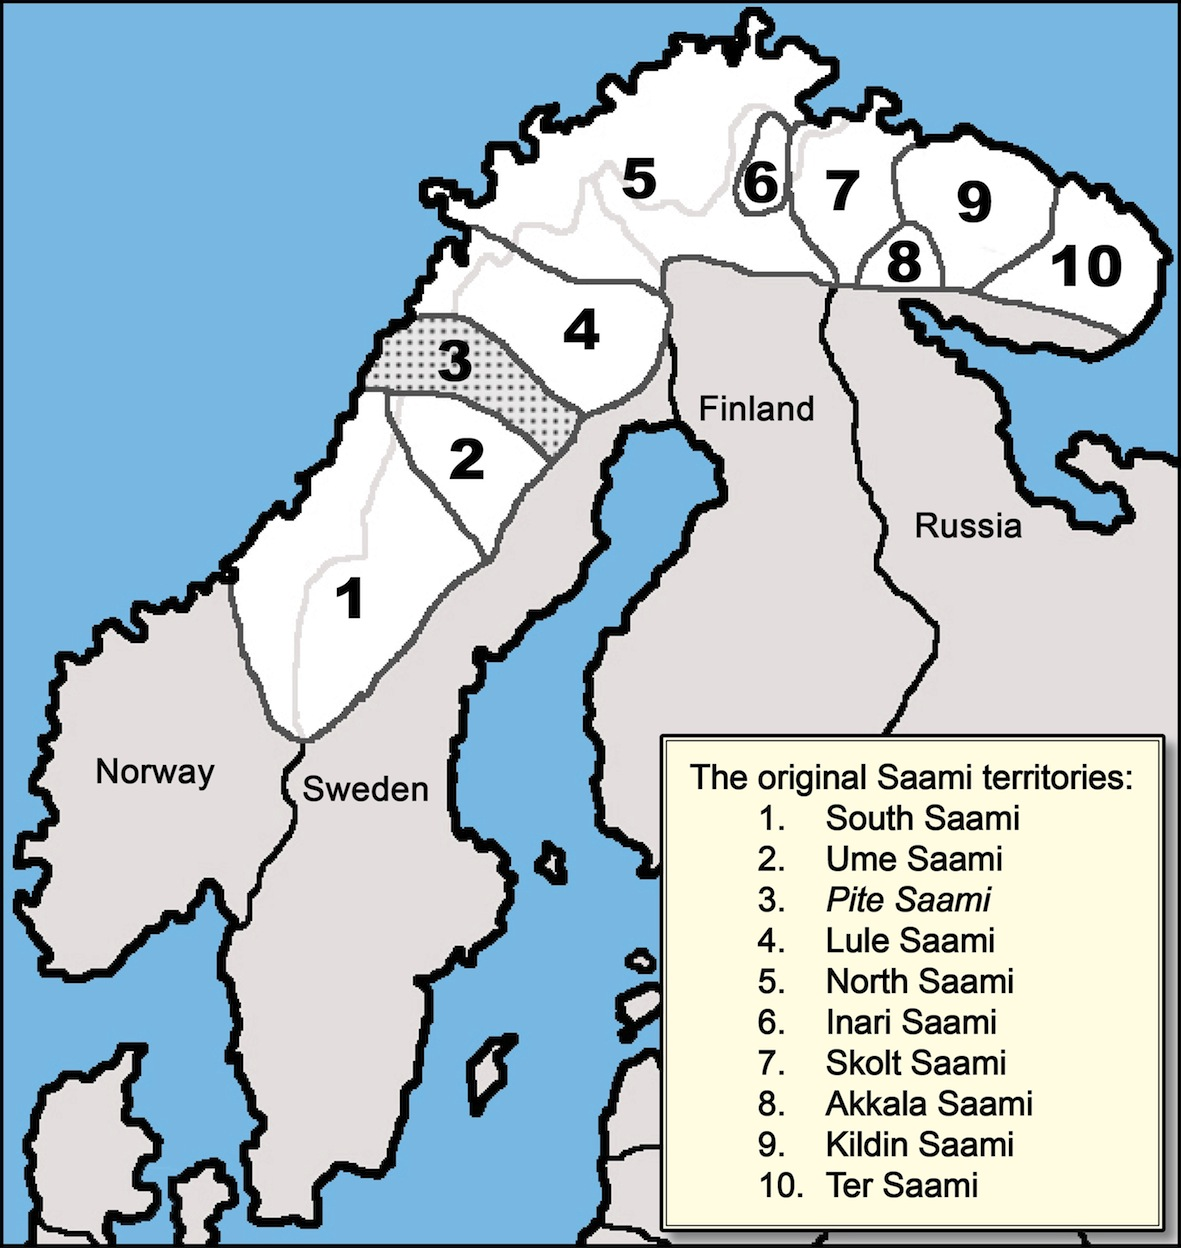
\includegraphics[width=.5\textwidth]{images/SaamiTerritoryMapPiteENsmall.jpg}
\caption[A map of \It{Sápmi}, the territory in which the Saami Languages were traditionally spoken]{A map of Sápmi, the territory in which the Saami languages were traditionally spoken, with \PS\ shaded in (borrowed from \mbox{\citealt[]{BullEtal2007}}, with permission)}\label{sabme}
\end{figure}

There is no official geographic or political unit defining any \PS\ linguistic or ethnic area, but the individuals (including both speakers and non-speakers) I have met, worked with or heard about who consider themselves to be \PS\ (regardless of language abilities) all come from an area based roughly on the Arjeplog municipality\footnote{Note that Arjeplog \It{municipality} (\It{kommun} in Swedish) refers to the larger administrative district of ca. 15,000 km\superS{2}, while the town of Arjeplog is the main village in the municipality.} 
in Swedish Lapland and bordering areas in Norway. On the Swedish side, this has traditionally been referred to as \It{Pite lappmark} ‘\PS\ territory’. 
For instance, Ruong, himself a native speaker of \PS, claims that the “most genuine form” (Ruong \citeyear[iii]{Ruong1943}; my translation) of the \PS\ language is spoken by members of the Luokta-Mavas \It{sameby},\footnote{A \It{sameby} (Swedish, literally ‘Saami village’; \It{samebyar} in \PL) is a group of reindeer herding families who tend their reindeer together in the same territory.} 
whose summer reindeer grazing lands are located along the headwaters of the Pite River, and by settled Saamis in the same area.\footnote{However, \citeauthor{Ruong1945} also included speakers from Semisjaur-Njarg \It{sameby} to the south as sources for his 1945 dissertation on verbal derivation in \PS. It is clear that Ruong is aware of the existence of the Saami dialect continuum and the \is{dialect variation}difficulty of drawing distinct language borders. He indicates that some areas on the north side of the Pite River drainage speak Lule Saami, while speakers along the Skellefte River drainage are more under the “influence of Southern Saami” (\citealt[iii]{Ruong1945}; my translation).} 
Manker’s ethnography of the Saami populations in the Swedish mountains \citep{Manker1947} outlines the three \It{samebyar} Luokta-Mavas, Semisjaur-Njarg and Svaipa as part of \It{Pite lappmark}.\footnote{\citet[473]{Manker1947} includes a map of all Swedish \It{samebyar} as a fold-out, and a map of these three \PS\ \It{samebyar}.} 
\citet[22]{Sammallahti1998} corroborates this, and adds the forest \It{sameby} Ståkke to the list. \citeauthor{Collinder1960} and \citeauthor{Bergsland1962} also help delineate the southern border of \PS\ territory. Collinder writes that the border “goes along the Pite River between the parishes of Jockmock [sic] and Arvidsjaur, and farther west through the parish of Arjeplog” (\citeyear[23]{Collinder1960}), while Bergsland further specifies that Ume Saami is spoken by “the forest Lapps in southern Arjeplog [...] and by the mountain Lapps in Sorsele” (\citeyear[27]{Bergsland1962}). %, thus drawing the southern border of \PS\ at essentially the same place. As for the Norwegian side, in researching his grammar, Lagercrantz (\citeyear{Lagercrantz1926}) worked with two \PS\ speakers whose families originated in the Arjeplog municipality but had resettled to the Beiarn area in Norway. 

As for the Norwegian side, some \PS\ reindeer herding families had their summer reindeer grazing lands in the Norwegian territory adjacent to the international border \cite[cf.][]{Manker1947}. The Finno-Ugrian scholar Eliel Lagercrantz worked with \PS\ speakers whose families originated in the Arjeplog municipality but had resettled to the Beiarn area in Norway \cite[cf.][]{Lagercrantz1926}. Ethnic \PS\ individuals still live in Norway, and are, for instance, still active in the local \PS\ association there, \It{Salten Pitesamisk Forening}. 

As a result, one can say that \PS\ was traditionally spoken in an area spanning both sides of the Norwegian-Swedish border around the municipality of Arjeplog on the Swedish side and across the border into Saltdal and Beiarn municipalities in Norway. %Reindeer herding \PS\ speakers still spend the winter months in the traditional reindeer grazing lands in the lowland forests along the Pite River drainage in Arvidsjaur and Älvsbyn municipalities in Sweden. 
On the Swedish side, the \PS\ area is essentially limited to the Pite River %(\It{Bidumedno}) 
drainage above the waterfall at Storforsen, and the sections of the Skellefte River %(\It{}) 
drainage from the town of Arjeplog and farther upriver. %to the north and south, respectively. 
The map in Figure \vref{piteTerritory} gives a rough idea of the traditional geographic area, which is the light area on the map. It is based on  \citet{Lagercrantz1926}, \citet{Ruong1943}, \citet{Manker1947}, \citet{Bergsland1962} and \citet{Sammallahti1998}, as well as on my own knowledge gained by discussing family histories with \PS\ individuals.

My own research indicates that \PS\ is currently still spoken by a few members of the Luokta-Mavas, Semisjaur-Njarg and Ståkke \It{samebyar}, as well as by settled Saami families from the same areas. Furthermore there are a few speakers from the Arjeplog municipality who have since moved to other areas outside of Arjeplog municipality, %such as along the northern Swedish coast, %(e.g., Luleå, Piteå, Umeå) 
even as far away as southern Sweden. %(e.g., Södertälje, Västerås and Norrköping). 
Ethnic \PS\ individuals from Norway have indicated to me that the last \PS\ speakers on the Norwegian side died several generations ago.%(Knut Sivertsen, p.c.). 

\setlength\fboxsep{0pt}
\setlength\fboxrule{1pt}
\begin{sidewaysfigure}
%\begin{figure}
\centering
\resizebox{\columnwidth}{!}{
\fbox{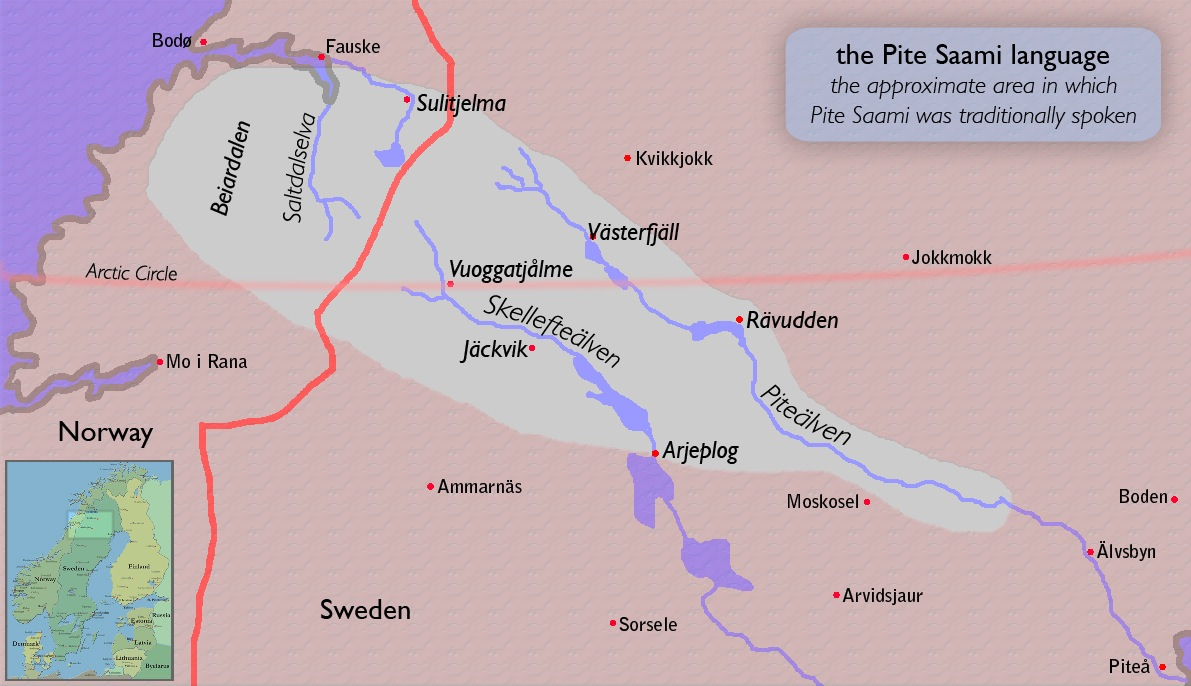
\includegraphics[width=1\textwidth]{images/piteTerritory.jpg}}}
\parbox{150mm}{\caption{An approximate map of the territory in which the \PS\ language was traditionally spoken\label{piteTerritory}}}%NOTE that label is inside caption! otherwise reference in text doesn’t work properly! (cf. http://www.leancrew.com/all-this/2008/09/latex-figure-captions/ )
%\end{figure}
\end{sidewaysfigure}%\end{landscape}

\FB
%\clearpage

\subsection{The state of the \PS\ language}\label{sociolinguistics}
Traditionally, most \PS\ families lived either as semi-nomadic reindeer herders or as sedentary farmers, fishers and hunters. Despite having always been in contact, these two groups lived very different lifestyles, and spoke Saami in relative isolation from one another. While reindeer herding Saami have often been a topic of Saami studies, the settled Saami are neglected or even actively prejudiced against for not being ‘true’ Saami since they do not herd reindeer. The data supporting the present study and gathered as part of the \PSDP\ (cf. \SEC\ref{PSDPcorpus}) originated from both groups.

By the eighteenth century, the Saami peoples had, in general, been converted from animistic polytheism to Christianity, marking the beginning of Saami assimilation to North Germanic culture \citep[cf.][]{Pulkkinen2005}. %\marginpar{how to cite this webpage?!? Cf. Missionary history of Lapland (Pulkkinen, Risto)} %\marginpar{add reference to “the encyclopedia of saami culture (presentation page: http://www.helsinki.fi/~sugl_smi/senc/en/esittely.htm) or other!}. 
Strict policies in the mid-nineteenth century sent \PS\ children to special ‘nomad schools’ where they were not allowed to speak Saami. Attending these schools also kept them away from their families and from regularly participating in \PS\ life, while reinforcing the state’s drive to exclusively promote Swedish\is{language contact} culture and social values \citep[cf.][]{ValijarviWilbur2011}. 

Accompanying this shift, traditional realms of \PS\ experience are slowly being left behind in favor of Swedish ones. With the introduction of modern conveniences, most \PS\ individuals have moved to permanent dwellings in populated communities, particularly Arjeplog, thereby leaving behind traditional ways of life. Along with this demographic shift, they are also losing the need to carry out traditional occupations using the \PS\ language. As a result, all \PS\ speakers today speak Swedish\is{language contact} fluently, and indeed use Swedish significantly more often in everyday life \citep[cf.][]{ValijarviWilbur2011}.

A gradual reverse in political and social policies in Sweden over the last decades led initially to the acceptance and then to the active promotion of multiculturalism, particularly concerning the Saami people. This has helped to positively change attitudes towards \PS\ identity. However, concerning the \PS\ language and many traditional cultural realms, this change seems inadequate for revitalization. For instance, the Swedish government's minority language law from 2010 only applies the blanket term \It{samiska} (‘the Saami language’), and, in doing so, completely disregards the reality that there are five different Saami languages in Sweden. Even within \It{Sápmi}, \PS\ is threatened by larger Saami languages, in particular by North Saami, which has an active speech community of around 30,000 speakers, regular television, radio, print and internet resources, and first-language instruction in public school \citep[cf.][209-211]{Salminen2007}. The robust status of North Saami in addition to the lack of an officially recognized \PS\ orthography allow local government agencies to conveniently support North Saami alone in fulfilling the language law's requirements; any positive effects on the \PS\ language are essentially negated.

According to my own data collected from \PS\ individuals during fieldwork, there are around 30 speakers left,\footnote{Cf. \citet[221]{Salminen2007}, who claims there are only 10 speakers, while the English abstract in \citet{Lehtiranta1992} erroneously claims that the \PS\ language is “now extinct.”} 
of around 2000 ethnic \PS\ individuals \citep[24]{Krauss1997}. With one exception, all speakers are older than 50. %See \SEC\ref{geography} for more on the area in which \PS\ is spoken. 
Based on my own observations, all speakers are fluent in the Swedish\is{language contact} language, even if many of them did not learn Swedish until they began school. Indeed, Swedish dominates everyday life for most speakers today, particularly for those who do not work in reindeer husbandry, and for those not living in the traditional \PS\ area. Only a few households (less than five) use \PS\ on a regular basis at home or in family situations, and these are still involved in reindeer husbandry. In public realms, the language is rarely used today. For a more detailed description and analysis of the situation the language is currently in, see \citet{ValijarviWilbur2011}.

\FB

\section{Linguistic documentation of \PS}\label{lingDoc}
The \PS\ language has been the subject of academic research in the past; cf. \citet{Halasz1896}, \citet{Lagercrantz1926}, \citet{Ruong1943} and \citet{Lehtiranta1992}. %, which are summarized in \SEC\ref{previousWork} below. 
This extant body of research was consulted in coming to terms with \PS\ linguistic structures in creating the present description. 
However, in fulfilling the goal of describing the \PS\ language as it is spoken in the early 21\superS{st} century, the \PSDP\ corpus, collected from 2008 through 2013, is the main source of data. With this in mind, I consider this a corpus-based description, as opposed to a literature-based description, which would have attempted to incorporate these previous works to a much greater extent. Indeed, everything not specifically cited as coming from another source is based on my own analysis of the corpus. 
The current description will hopefully be seen as a supplement to previous work on \PS, and together with previous studies, can facilitate exploring language change as exemplified by a severely endangered language. 

In the following sections, previous studies on \PS\ are summarized in \SEC\ref{previousWork}. The current corpus and the documentation involved in creating it are described in \SEC\ref{PSDPcorpus}. Then \SEC\ref{usingThis} provides a short guide to using this description. 

\subsection{Previous studies}\label{previousWork}
%The\marginpar{check this entire first paragraph!} first written \PS\ texts were likely collected by Hungarian scholar Jozséf Budenz in 1873 in Budapest. Budenz worked with four Saami men who were part of a so-called \It{human zoo} exhibition. The men were from ‘Pite Lappmark somewhere beyond Skellefteå’ (\citealt[161]{budenz1876a}; my translation). Budenz’ article \It{Svéd-lapp nyelymutatványok}\footnote{ ‘Swedish-Lappish language samples’.} \citep{budenz1876a} includes small anecdotes, short Bible translations, and a word list with Hungarian translations. The actual origin of the four men is unclear, but the texts seem to be in \PS. 
%
In the late 19\superS{th} century the Hungarian scholar Ignácz Halász studied \PS, and wrote several studies in Hungarian on the language. 
\It{Lule- és Pite-lappmarki nyelvmutatvéanyok és szótár}\footnote{‘Linguistic examples and a wordlist from Lule and \PS\ territory’.} \citep{Halasz1885} contains the Gospel of Matthew in Lule Saami, and a combined Lule Saami/\PS\ wordlist with translations in Hungarian and German. 
\It{Népköltési gyüjtemény: a Pite Lappmark Arjepluogi egyházkerületéböl}\footnote{‘Collection of traditional verses from the bishopric of Arjeplog in \PS\ territory’.} \citep{Halasz1893} 
consists of a significant text collection of short \PS\ texts, transcribed using the traditional Finno-Ugrian transcription. Each text is translated as a whole into Hungarian. The majority of the texts are traditional narratives, %including some ‘stallo’ (a large, stupid creature common in Saami mythology) stories, 
and a few poems and songs are also transcribed and translated. 
\It{Pite lappmarki szótár és nyelvtan}\footnote{‘Wordlist and grammatical description from \PS\ territory’.} \citep{Halasz1896} 
includes morphological paradigms and a \PS\ wordlist with translations into Hungarian and German. 

\It{Sprachlehre des Westlappischen nach der Mundart von Arjeplog}\footnote{‘A grammar of West Saami based on the Arjeplog dialect’.} \citep{Lagercrantz1926} 
is a grammar in German. It is based on three months of fieldwork during which Lagercrantz consulted three \PS\ individuals who had settled in the Beiarn district in Norway but who were originally from the Arjeplog municipality. The book covers semantically driven descriptions of clause structures, a limited description of morphology, and an extended analysis of the phonological system, based on phonetic acoustic experiments. 

\It{Lappische Verbalableitung dargestellt auf Grundlage des Pitelappischen}\footnote{‘Saami verbal derivation as illustrated by \PS’.} \citep{Ruong1943} is the dissertation of Israel Ruong, who later became professor of Saami languages and culture at Uppsala universitet. Ruong’s native language was \PS; his dissertation, an elaborate categorization of \PS\ verb derivations, is his only study specifically dealing with the \PS\ language. %His dissertation is an elaborate categorization of \PS\ verb derivations. %\marginpar{better description of Ruong1943!}.

\It{Arjeploginsaamen äänne- ja taivutusopin pääpiirteet}\footnote{‘The fundamentals of Arjeplog Saami phonology and inflection’.} \citep{Lehtiranta1992} is a Fin\-nish-language description of \PS\ phonology and inflectional patterns, and is based on recordings, publications and archived materials on \PS\ from 1950 and earlier. Some paradigms can be found at the end of the book, as well as several \PS\ texts with phonetic and orthographic transcriptions, as well as Finnish translations. The phonetic transcriptions are presented in the transcription standard used in Finno-Ugrian studies. 

Note that these studies deal with \PS\ as it was spoken before 1950. Finno-Ugristian studies have traditionally dealt with historical-comparative studies, and have not always been concerned with the synchronic state of Saami languages. Indeed, the distance some scholars keep from the synchronic situation is highlighted by the erroneous claim by Lehtiranta %, as pointed out in a previous footnote, 
that \PS\ is “now extinct” \citep[English abstract]{Lehtiranta1992}. 
Consequently, the present study is the first extensive description of the \PS\ language in English and for a general linguistic audience. % are just now becoming available as a result of the \PSDP\ and the present PhD thesis.%

Since the present study is intended to be a synchronic description of the \PS\ language as used in the early 21\superS{st} century and reflected by the \PSDP\ corpus, the previous work mentioned above have played an indirect but important role in its creation. However, these works were referred to in detail particularly when the data from the corpus were not substantial enough to allow relatively certain conclusions to be drawn. Data based at least partly on sources other than the documentation corpus are clearly marked as such in this description. Specifically, the sections in \mbox{\citet{Lagercrantz1926}} concerning phrasal and sentence-level syntactic phenomena in Part A ‘\It{Ausdruckslehre}’ (pp. 19-99) were informative, while Part B ‘\It{Formenlehre}’ (pp. 103-141), the paradigms throughout \citet{Halasz1896} as well as the paradigms in the appendix to \citet[150-166]{Lehtiranta1992} were consulted regarding morphology. In writing Chapter \ref{derivMorph} on derivational morphology, Ruong’s thesis  (particularly Chapters 6 through 40, which present his data) provided valuable insights into the variety and complexity of \PS\ derivation from both morphological and semantic perspectives. %; particularly Chapters 6 through 40, which present his data, were considered.

In addition to the academic linguistic studies mentioned above, a number of other texts exist concerning the \PS\ language and its people. \citet{ValijarviWilbur2011} describe the current state of the \PS\ language from the  point of view of sociology of language. \citet{sjaggo2010a} deals with the etymology of a selection of \PS\ place names along the river Piteälven in the Arjeplog municipality. 
A large number of \PS\ \It{vuole}\footnote{This is nominative plural; the nominative singular form is \It{vuolle}.} 
(songs in the Saami singing tradition of \It{yoik}) were recorded in the first half of the 20\superS{th} century. These can be found transcribed in a number of works: 
\citet{tiren1942a} includes 139 transcriptions of \PS\ melodies and lyrics, with German translations; 
\citet{grundstroem1958a} have 93 songs by Jonas Eriksson Steggo in the form of transcribed melodies and lyrics, with translations in Swedish and German; 
\citet{grundstroem1963a} provide 73 songs by a variety of \PS\ individuals in the form of transcribed melodies and lyrics, also with translations in Swedish and German.
%are covered in part in \citet{stoor2007a}. 
\citet{wickman1964} discusses a short \PS\ text from a recording done in 1939 by Israel Ruong; the text is presented in three transcription standards (Finno-Ugrian close phonetic standard, the author’s own phonemic transcription, and a modified North Saami orthography) and includes an English translation. 
Lars Rensund’s books (\citeyear{Rensund1982}, \citeyear{Rensund1986}) detail personal recollections by the author, himself a Pite Saami, and are interspersed with sentences and occasionally  entire narratives in \PS. \citet{bylund1956} provides an in-depth study of the colonization of \PS\ territory by Swedish\is{language contact} settlers up to the middle of the 19\superS{th} century. 
No educational materials, bible translations or other common texts exist in the \PS\ language. With the exception of the works by Lars Rensund, most \PS\ speakers today are not aware of any of the works mentioned above. 



\subsection{The \PSDP\ corpus}\label{PSDPcorpus}
%\section{The \PSDP\}
The data forming the basis of the present study were collected as a part of the \PSDP. This description is a direct result of that project, the main goal of which is the linguistic documentation of the \PS\ language. The project has so far resulted in audio and video recordings documenting current language usage and grammatical structures and includes an archived corpus comprising 29,208 transcribed and translated \PS\ words (as of early March 2014; %January 2013, the \PSDP\ corpus consists of 25,227 %25,227+1815 (added in May 2013)=27042
%transcribed and translated \PS\ words.} %of those recordings and relevant transcriptions and annotations 
cf. the \hyperlink{inventoryRef}{Appendix} for a list of recordings). 
From June 2008 until July 2011, the project was carried out by Joshua Wilbur at the Nordeuropa-Institut at Humboldt-Universität zu Berlin, with support from the \href{http://www.hrelp.org/grants/}{Endangered Languages Documentation Programme} (ELDP; a part of the Hans Rausing Endangered Languages Project, with financial support from the Arcadia foundation and hosted by the School for Oriental and African Studies (SOAS) at the University of London). %Funding consisted of GBP 64,748 over the course of the project to support fieldwork, equipment expenditures, payments for language consultants and to cover a graduate student stipend. 
A continuation of the project is underway in 2013 and 2014 at Albert-Ludwigs-Universität Freiburg thanks to generous continued funding from ELDP. 

Current trends in documentary linguistics\is{documentary linguistics} were taken into account.\footnote{Cf. \citet{BirdSimons2003}, \citet{Gippert2006}, \citet{Woodbury2011}, \citet{AustinSallabank2011}, \citet{GrenobleFurbee2010}, the book series \It{Language Documentation and Description}, among others.} 
Himmelmann’s proposal that “a language documentation is a lasting multipurpose record of a language” \citep[1]{Himmelmann2006a} is a defining motivation behind the project. Accordingly, the resulting documentation consists of a documentation corpus of a variety of linguistic genres, including \PS\ situations potentially of interest to non-linguistic disciplines and to members of the \PS\ language community themselves, as well as the present description. Initial results have been archived at five archives at international, national, regional and local levels:
\begin{itemize}
\item{\It{The Endangered Languages Archive} (ELAR) at the School for Oriental and African Studies in London;}
\item{\It{The Language Archive} at the Max Planck Institute for Psycholinguistics in Nijmegen;}
\item{\It{Dialekt-, ortnamns och folkminnesarkivet i Umeå}\footnote{‘The Department of Dialectology, Onomastics and Folklore Research in Umeå’.} (DAUM) in Umeå, Sweden;}
\item{\It{Ájtte: Svenskt Fjäll- och Samemuseum}\footnote{‘Ájtte: the Swedish Mountain and Saami Museum’; \It{ájtte} is the Lule Saami word for a traditional Saami storage shed.} in Jokkmokk, Sweden;}
\item{\It{Silvermuseet}\footnote{‘The Silver Museum’.} in Arjeplog, Sweden.}
\end{itemize}
Working with multiple archiving sites as well as having all data in a digital format help ensure accessibility to and longevity of the data. 

Access to the materials is available via the archives (in some cases, this is possible via the world wide web). %, assuming adherence to access protocol on a file-by-file basis. 
Ideally, an archive should provide interested parties with access to archived materials, while respecting the privacy and the wishes of recording participants as necessary; with this in mind, access rights to the data related to any given session reflect the wishes of speakers involved in a specific session concerning availability to the linguistics and other scientific communities, the \PS\ and greater Saami communities, and other individuals and groups in general. %Any commercial use of the materials is strictly prohibited. 
Furthermore, as part of a scientific endeavor, the claims made in this book about \PS\ linguistic structures should be reproducible; with this in mind, the original data are available to the academic community via the Language Archive at the Max Planck Institute for Psycholinguistics in Nijmegen, the Netherlands; see \SEC\ref{archiveAccess} for more details on accessing the archive. 
%In adhering to good scientific practice, claims based on \PS\ data and presented here should be reproducible by 
%Specifically regarding this grammatical description as presenting scientifically sound and reproducible linguistic results, access to the corpus is available to the academic community via the archive at the Max\,Planck Institute for Psycholinguistics in Nijmegen, the Netherlands; see \SEC\ref{archiveAccess} for more details on accessing the archive. 


\subsubsection{Collection methods}\label{collectionMethods}
Data were collected and recordings were transcribed during a total of 23 months at the field site in and around Arjeplog, Sweden, %Over the course of field work, I was able to develop productive working as well as personal relationships with several native speakers of \PS\ interested at least passingly in documenting their language. 
with the invaluable assistance of a number of \PS\ speakers. They were compensated for their time and effort with a modest consultant honorarium. 

The documentation corpus consists of more than 55 hours of recordings covering a variety of genres; cf. the Appendix for a list of recordings, including an indication of genre and medium. 
As the morphological structure of \PS\ words is quite complex, %(e.g.~17 word forms in a noun paradigm, at least 24 in a verb paradigm), 
it was necessary to rely on elicitation techniques to gather a sufficient number of word forms for a wide variety of lexemes as a basis for morphological analyses. 
As a result, the majority of recordings (approximately 45 hours) consist of elicitation sessions intended to gather specific details concerning the structure of the language. 
These were often conducted using Swedish as a metalanguage, but \PS\ was used whenever efficient and useful, and more frequently in recordings made later in the project. 
A variety of elicitation methods were used. To a large extent, elicitation sessions were conducted as translational interviews (particularly in early recordings to collect initial wordlists) and sentence completion (using both Swedish and \PS\ triggers, mostly to complete morphology paradigms). However, other methods were used as well, such as vocabulary card ordering tasks to test syntactic structures, and tasks using toy blocks to gather data on spatial relations. 
Many non-elicitation linguistic situations were also recorded, covering genres such as conversations, explanations, narrations, performances, as well as songs and readings; in the current documentation corpus, such recordings comprise approximately 17,700 transcribed words. A few written texts were also collected to supplement recordings. 

Each collection of materials\footnote{Note that the archive at the Max Planck Institute for Psycholinguistics in Nijmegen, the Netherlands, refers to the entire collection of files concerning a single recording as a ‘session’, not a ‘collection’.} 
in the corpus corresponds to a recorded linguistic event. Each collection has a unique name based on the pattern:
\begin{center} pitYYMMDDabc \end{center}
(pit = \PS, YYMMDD = abbreviated date of recording with a two-digit year, abc = further disambiguation as needed). Recordings done for the project from 2012 onwards use the ISO 639-3 code \It{sje} as a prefix for session names instead of \It{pit}, and a four-digit year; e.g.,~{sje2012}1014b. 
All digital files related to a certain collection are named based on this pattern. 

In almost all cases, the following recording equipment, standards and software were used for documentation. A small number of deviations exist, and are indicated in the archived metadata for the relevant sessions. 
 
\Bf{Video}: a Panasonic NV-GS500EG-S video camera using miniDV cassettes in short play (SP) mode, using a wide-angle lens attachment and a tripod. In most cases, a RØDE SVM stereo video microphone was mounted on the camera for audio in place of using the built-in microphone.

\Bf{Audio}: an Edirol R-09 digital audio recorder set to record 16-bit WAV format at 44.1 kHz. A variety of microphones was used, depending on the specific recording situation; these included a RØDE SVM stereo video microphone, a Sennheiser lapel microphone connected to a Sennheiser EW 112-p G2 wireless set and a Sennheiser MKE 300 shotgun microphone. %, and a Sony ECM-MS957 shotgun microphone. %JW: this is Micha’s and Florian’s mic

\Bf{Still images}: a Canon IXUS 80IS digital photo camera was used to take digital photographs to supplement documentation. Images are in JPEG format.

\Bf{Editing/Computing}: video/audio recordings were transferred to a Macintosh MacBook Pro for further editing, as necessary. Video was edited using Final Cut Express and Final Cut Pro software. Audio was archived in the original quality, while video was compressed to MPEG-2 or MPEG-4 format.

\Bf{Transcribing/annotating}: the multimedia annotation program ELAN\footnote{ELAN is free software developed by the Technical Group of the Max Planck Institute for Psycholinguistics (see \href{http://www.lat-mpi.eu/tools/elan/}{www.lat-mpi.eu/tools/elan/}).} 
was used to transcribe and annotate recordings. Annotation/transcription files are archived in both ELAN format and in plain text format.


Initial transcriptions of recordings were completed with the help of native speaker assistants.\footnote{I am particularly indebted to Elsy Rankvist for her invaluable transcription assistance.} 
Transcriptions in the corpus are written in various versions of the \PS\ orthography under development by the wordlist project \It{Insamling av pitesamiska ord} (cf. \SEC\ref{orthography}),  %carried out by members of the \PS\ language community. At the time of writing, the project’s orthographic standards have not been fully finalized nor recognized by any official authority. 
but have been standardized according to the principles explained in \SEC\ref{orthography} when cited in this book. 
All transcribed words are provided with annotations in the form of at least a translation into English or Swedish or as morpheme-by-morpheme glosses. Such glosses can serve as the sole translation of a transcribed word or utterance, particularly for data from transcribed elicitation sessions. Both glosses and free translations into English and/or Swedish may be provided, especially in non-elicited text genres. Relevant notes or commentary may also exist as annotations. 

Metadata were collected in a database using the FileMaker Pro program, then exported to XML and plain text formats for archiving. Information collected concerns participants, the recording situation, location, equipment used and a summary of the contents of the recording, among other things.

\nopagebreak[4]
Any given collection consists minimally of the following set of digital files: %\footnote{in one case (pit090515), there is no audio recording, but instead a written text, and no additional transcription/annotation files.}
%\vbox{%keeps items from crossing pagebreak (but moves next figure to bad place here, thus commented out)
\begin{itemize}
\item{audio recording in WAV format (16-bit, 44 kHz)}
\item{transcription/annotation file in ELAN and in plain text format}
%\item{transcription/annotation file in plain text format}
\item{metadata concerning the session in XML and plain text formats}
\item{metadata concerning the entire collection in XML}
%\item{}
\end{itemize}
In addition to the above files, collections may also include the following files:
\begin{itemize}
\item{video recording in MPEG-2 or MPEG-4 format}
\item{digital images in JPEG format}
\item{other supplementary files}
\end{itemize}
%}

The transcription/annotation files are divided into numbered, utterance-based units and include at least a transcription of any \PS\ language usage. 
A specific utterance can be referred to using the collection/session name and the utterance number. 
The \PS\ original is translated into Swedish and/or English, and provided with linguistic glosses. Other comments are included as well, whenever deemed relevant or useful. 
Finally, in cases with code-switching, the language being used in a certain utterance, or part thereof, is indicated. Tiers in all ELAN files are organized hierarchically based on the template %illustrated %removed to keep extra line from being added in final formatting!
in Figure \vref{ELANhierarchy} for each speaking participant in a recording, plus a ‘notes’ tier for general comments. %\marginpar{or should this be considered a Table?}.
 A list of all recordings in the corpus can be found in the Appendix on page \pageref{inventory}, including brief descriptions of content and an indication of the number of \PS\ words transcribed and translated per recording. 
\newcommand{\Descr}{30mm}%variable to set x-axis length for tier descriptions
\begin{figure}[h]\centering
%\resizebox{\columnwidth}{!}{%
\begin{tikzpicture}
\draw [blue,ultra thick] (-3mm,0mm)--(6mm,0mm) node[anchor=west,black]{ref};
\draw [blue,ultra thick] (5mm,0mm)--(5mm,-30mm)--(11mm,-30mm) node[anchor=west,black]{lang};
\draw [blue,ultra thick] (5mm,-25mm)--(11mm,-25mm) node[anchor=west,black]{nt};
\draw [blue,ultra thick] (5mm,-5mm)--(11mm,-5mm) node[anchor=west,black]{text};
\draw [blue,ultra thick] (10mm,-10mm)--(16mm,-10mm) node[anchor=west,black]{ftrLing};
\draw [blue,ultra thick] (10mm,-15mm)--(16mm,-15mm) node[anchor=west,black]{ftrE};
\draw [blue,ultra thick] (10mm,-5mm)--(10mm,-20mm)--(16mm,-20mm) node[anchor=west,black]{ftrS};
\draw [blue,ultra thick] (-3mm,-35mm)--(6mm,-35mm) node[anchor=west,black]{notes};
\draw [font=\itshape,red,ultra thick,densely dashed] (-3mm,-35mm)--(-3mm,1.8mm) node[anchor=south]{root};%root bar
\draw (\Descr,0mm) node[font=\footnotesize,anchor=west]{Assigns each utterance a number and time alignment};
\draw (\Descr,-5mm) node[font=\footnotesize,anchor=west]{Transcription of utterance in \PS\ orthography};
\draw (\Descr,-10mm) node[font=\footnotesize,anchor=west]{Linguistic glossing};
\draw (\Descr,-15mm) node[font=\footnotesize,anchor=west]{Free translation in English};
\draw (\Descr,-20mm) node[font=\footnotesize,anchor=west]{Free translation in Swedish};
\draw (\Descr,-25mm) node[font=\footnotesize,anchor=west]{Notes on the utterance};
\draw (\Descr,-30mm) node[font=\footnotesize,anchor=west]{Language used};
\draw (\Descr,-35mm) node[font=\footnotesize,anchor=west]{General comments};
%\draw [black] (-8mm,7mm)--(103mm,7mm);%header line
%\draw [black] (-8mm,-38mm)--(103mm,-38mm);%footer line
\draw (9mm,9.4mm) node[font=\footnotesize,anchor=west]{tier name};
\draw (-8mm,9mm) node[font=\footnotesize,anchor=west]{hierarchy};
\draw (\Descr,8.7mm) node[font=\footnotesize,anchor=west]{purpose};
\end{tikzpicture}%}
\caption{ELAN tier hierarchy used in the documentation corpus}\label{ELANhierarchy}
\end{figure}

%\FB


\subsection{Using this description}\label{usingThis}  
This description of the grammar and the accompanying documentation corpus are together intended to outline the structural features of the \PS\ language and provide an empirical foundation for claims made in the present work. In addition, the documentation should give interested individuals (linguists, Saami individuals, etc.) the opportunity to explore other aspects of the language as well. Finally, it should also secure a record of the language as spoken by those \PS\ individuals who likely comprise the last generations of speakers for future generations of ethnic \PS\ individuals. 

The following sections are meant to assist in utilizing both the description and the accompanying documentation corpus. 
The first section (\SEC\ref{accountabilityEtc}) deals with accountability and verifiability, while the second section (\SEC\ref{archiveAccess}) provides brief instructions on how to access data from the corpus. 
Then, \SEC\ref{examplesExample} illustrates how examples from the corpus are presented. %, and \SEC\ref{organizationalPrinciples} briefly discusses the organizing principles used to structure the grammatical description. 
Finally, \SEC\ref{orthography} covers orthographic considerations and includes a list of phonemes and the graphemes used to represent these. 
A list of symbols and abbreviations used in the present work is provided starting on page \pageref{symbolList}. 


\subsubsection{Accountability and verifiability}\label{accountabilityEtc}
Data in the present study are cited with a bracketed reference to the collection name followed by the specific utterance number or timecode within a recording. 
This should allow the reader to easily find the evidence cited and make his/her own judgement about the conclusions made. References to specific recordings marked with ‘\It{e}’ after the closing bracket indicate that the presented utterance was attained during an elicitation session. 
For instance, the reference 
\begin{center}\small[pit090930a.239]\It{e}\end{center}
refers to utterance number \It{239} on recording \It{pit090930a}, and indicates that this example is from an elicitation session. %(made on 24\superS{th} September 2008). 

In order to verify, scrutinize or otherwise review the actual primary data on which the present study is based, the data can be accessed via one of the archives listed in \SEC\ref{PSDPcorpus}. Specific instructions are provided in the following section. 


\subsubsection{Accessing archived materials}\label{archiveAccess}
The archivists at the IMDI archive located at the Max Planck Institute for Psycholinguistics in Nijmegen, the Netherlands, have kindly agreed to host the \PSDP\ spoken language corpus. For those interested in accessing the data in connection with the present description, I recommend using this archive. \PS\ materials are available via the on-line IMDI-browser at: 
\begin{center}\href{http://corpus1.mpi.nl/ds/imdi_browser/}{corpus1.mpi.nl/ds/imdi\_browser/}
\end{center}
under the hierarchical node:
\begin{center}\href{http://corpus1.mpi.nl/ds/imdi_browser/?openpath=MPI1565580\%23}{ Endangered Languages/Donated Corpora/Pan-Saami Language Archive/Pite}
\end{center}


\subsubsection{Explaining examples}\label{examplesExample}\hypertarget{explExs}
Examples from the corpus are numbered consecutively for easy reference, and consist of several lines of text. The spoken text is presented in italics in the initial line in the orthographic standard, followed by interpretive information in the form of a morpheme-by-morpheme breakdown in the second line and English glosses in the third line. Finally, the last line contains a free translation in English and a reference to the source recording in the corpus; this reference includes either the number of the specific utterance or its initial time code.\footnote{A source recording reference followed by ‘\It{e}’ indicates that the example shown was from elicited data; cf. \SEC\ref{accountabilityEtc}.} 
Examples are formatted as shown in Figure \vref{exampleExplanation}.
\begin{figure}[h]
\hspace{-10pt}\begin{tabular}{p{.07\columnwidth} p{.89\columnwidth}}
(no.)&\It{\PS\ original text}\\
	& \PS\ text with morpheme boundari-es\\
	& Morpheme-by-morpheme glossing \\%\Sc{with grammatical categories in small caps}\\
	& ‘free English translation’\hbox{}\hfill{\small\textnormal{[source]}}\\ %\hspace*{200pt} \small\textnormal{[source]}\normalsize
\end{tabular}
\caption{Template used in examples of utterances}\label{exampleExplanation}
\end{figure}

In Chapter \ref{ProsodicStructure} on prosody and Chapter \ref{csANDvs} on segmental phonology, many examples of individual words are provided to illustrate phonological aspects of \PS. In most cases, the phonological representation and phonetic realization (both using IPA standards) and the orthographic representation (based on the current working version) are included, as well as a gloss and a reference to the source recording, as summarized in Figure \vref{exampleExplanationWords}. In such examples, the phonemic representation also indicates any linear morpheme boundaries. 
\begin{figure}
(no.)\hspace{1em}
\begin{tabular}{p{30mm} l}
/phonem-ic/ 		& \It{orthography}	\\%\MR{2}{*}{\hfill\small[source]} \\
\MC{1}{l}{[phonetic]}	& ‘gloss’			\\
\end{tabular}\hfill\small[source]
\caption{Template used in examples for individual words}\label{exampleExplanationWords}
\end{figure}
%\noindent 
%\label{wordlistReference}
The source recording for these words indicates the recording name and utterance number or time code in most cases. However, when only a four-digit number is present (e.g.,~{\small[0457]}), this indicates that the original recording is not from the documentation corpus, but from the Wordlist Project (cf. \SEC\ref{orthography}). The number refers to the record number of the word in the Wordlist Project’s lexical database, and the accompanying recording of that specific wordlist item, as collected by the members of the Wordlist Project. Currently, the recordings of the entries in the wordlist have not been archived, but will likely be archived in the near future once the permission of the members of the Wordlist Project has been secured. Some examples in Chapter \ref{derivMorph} on derivational morphology are also from this lexical database, and are marked in the same way. 


\subsubsection{Orthographic considerations}\label{orthography}\is{orthography|(}
At the time of writing, \PS\ does not have an officially recognized orthography. In the past, adapted versions of the Swedish\is{language contact} orthographic standards\footnote{Cf. Lars Rensund’s books (\citeyear{Rensund1982,Rensund1986}).} 
and Lule Saami orthographies\footnote{E.g., at literacy courses for \PS\ individuals held in Arjeplog occasionally during the last decade and sponsored by the Swedish Saami Parliament.} 
have been used to write \PS\ for a non-technical, non-linguistic audience. However, from 2008 through 2011, \It{Arjeplogs sameförening} (the local Saami association in Arjeplog) received funding to complete a lexicographic project called \It{Insamling av pitesamiska ord},\footnote{This translates roughly as “collecting \PS\ words”. A working version of the resulting lexical database is currently available online at: \href{http://saami.uni-freiburg.de/psdp/pite-lex/}{http://saami.uni-freiburg.de/psdp/pite-lex/}.} 
%\href{http://gtweb.uit.no/webdict/index_sje-swe.html}{http://gtweb.uit.no/webdict/index\_sje-swe.html}.} 
\citep[cf.][]{insamlingPS2011} 
and hereinafter referred to simply as ‘the \WLP’. 
One of the outcomes of the \WLP\ was a working orthography for \PS. 
%As part of the \PS\ Documentation Project, I worked closely with the members of the \WLP\ as an unofficial linguistics consultant and 
I have attempted to adopt this working orthographic standard in writing \PS\ data in this description and the transcriptions provided in the accompanying documentation. This orthography uses the Swedish alphabet and many Swedish sound-to-grapheme correspondences, but also resembles to some extent Lule Saami orthographic systems, particularly the most recent one as found in \citet{KorhonenO2005}. To help understand the orthography, the correlations between sounds and graphemes are discussed here and listed in Table \ref{orthTableC} starting on page \pageref{orthTableCbegin} for consonants, and in Table \vref{orthTableV} for vowels. %\marginpar{this table was just copied in - it needs to be re-worked, checked!!!}
Chapter \ref{csANDvs} describes the segmental phonology represented by these graphemes in detail. 
An orthography proposal for the \PS\ language, including a more thorough description of these rules, is currently being put together by the members of the \WLP\ and the \PSDP, and is scheduled to be published, together with the \WLP’s wordlist, in late 2014 with funding from Arjeplog municipality. 

It is important to note that the standards used in this book are based on a \It{working} orthography, i.e., it is still subject to inconsistencies and potentially to further refinement. Moreover, the following description and the implementation of the orthography is based on my interpretation of the recurring patterns used by the \WLP\ in developing the orthography proposal mentioned above. While I generally use the spellings found in the \WLP’s wordlist, some deviations may be found in this description and the accompanying transcriptions; these can be due to a variety of factors such as changes to the wordlist as it was developed, deviating analyses on my own behalf, or simple inconsistencies in spelling (a natural occurrence in the development of an orthography) in the source. However, I alone am ultimately responsible for the orthographic choices in the present work. 

The unaspirated singleton plosive phonemes are normally represented by the graphemes <b>, <d> and <g>, except as a single word-final consonant, in which case <p>, <t> and <k> are used; this is illustrated for the alveolar plosive phoneme /t/ in \REF{spellExPlos1a} through \REF{spellExPlos1c}. 
\ea\label{spellExPlos1a}
\SpellEx{\Bf{d}állve}{\Bf{t}aːlːve}{winter}
\z
\ea\label{spellExPlos1b}
\SpellEx{bå\Bf{d}av}{pɔ\Bf{t}av}{come (\Sc{1sg.prs})}
\z
\ea\label{spellExPlos1c}
\SpellEx{båhte\Bf{t}}{pɔʰte\Bf{t}}{come (\Sc{inf})}
\z

The affricate phonemes are represented by the digraphs <ts> and <tj>; this is illustrated in \REF{spellEx0a} and \REF{spellEx0b}. 
\ea\label{spellEx0a}
\SpellEx{\Bf{ts}igget}{\Bf{ʦ}igːet}{set up}
\z
\ea\label{spellEx0b}
\SpellEx{alma\Bf{tj}}{alma\Bf{ʧ}}{person}
\z

In general, geminate consonants are written by doubling the relevant grapheme, as illustrated in \REF{spellEx1} through \REF{spellEx3}. 
\ea\label{spellEx1}
\SpellEx{gå\Bf{dd}et}{kɔ\Bf{tː}et}{kill}
\z
\ea\label{spellEx2}
\SpellEx{ká\Bf{ff}a}{kaː\Bf{fː}a}{coffee}
\z
\ea\label{spellEx3}
\SpellEx{ma\Bf{ŋŋ}el}{ma\Bf{ŋː}el}{after}
\z
However, geminate segments represented by digraphs, such as <sj> for /ʃ/ or <tj> for /ʧ/ %\marginpar{technical term for ‘a combination of letters’?} 
are written by doubling the initial grapheme, as in \REF{spellEx4} through \REF{spellEx5b}.
\ea\label{spellEx4}
\SpellEx{bå\Bf{ssj}o}{pɔ\Bf{ʃː}o}{kitchen}
\z
\ea\label{spellEx5}
\SpellEx{ma\Bf{nnj}e}{ma\Bf{ɲː}e}{daughter-in-law}
\z
\ea\label{spellEx5b}
\SpellEx{gå\Bf{ttj}åt}{kɔ\Bf{ʧː}ɔt}{urinate}
%\SpellEx{i\Bf{ttj}i-j}{i\Bf{ʧː}ij}{\Sc{neg}-\Sc{3sg.pst}}
\z

Preaspiration is represented by <h> when the preaspirated segment is the initial segment in the consonant center (cf. \SEC\ref{CCent}), as in \REF{spellEx6} and \REF{spellEx7}. 
%For preaspirated geminates, the aspiration is represented by <h>, while the long consonant is indicated by doubling the relevant letter, as in \REF{spellEx6} through \REF{spellEx7}. 
\ea\label{spellEx6}
\SpellEx{bå\Bf{ht}et}{pɔ\Bf{ʰt}et}{come}
%\ea\label{spellEx6b}
%\SpellEx{mä\Bf{htts}e}{mɛ\Bf{ʰʦː}e}{forest}
%%\SpellEx{ä\Bf{htts}et}{ɛ\Bf{ʰʦʦ}et}{love}
\z
\ea\label{spellEx7}
\SpellEx{á\Bf{httj}e}{aː\Bf{ʰʧː}e}{father}
\z
If a preaspirated segment is preceded by a sonorant consonant segment, then the preaspiration itself is not marked by a grapheme of its own, as in \REF{spellEx8} through \REF{spellEx10}.
\ea\label{spellEx8}
\SpellEx{mu\Bf{rrk}o}{mu\Bf{rːʰk}o}{fog}
\z
\ea\label{spellEx9}
\SpellEx{gu\Bf{mmp}e}{ku\Bf{mːʰp}e}{wolf}
\z
\ea\label{spellEx10}
\SpellEx{vua\Bf{nnts}a}{vu͡a\Bf{nːʰʦ}a}{hen}
\z
For plosives, the preaspiration is evident nonetheless because the corresponding plain segments are spelled differently, using <b, d, g>. However, the current working version of the orthography does not provide a way to distinguish between preaspirated affricates preceded by a sonorant segment, e.g.,~\REF{spellEx10}, and plain affricates preceded by a sonorant segment. 
%\begin{exe}
%\ea\label{spellEx11}
%\SpellEx{vua\Bf{nnts}a}{vu͡a\Bf{nːʰʦ}a}{hen}
%\z

In spoken \PS, when the copular and auxiliary verb \It{lä} is preceded by a word ending in an open syllable, it is often encliticized as \It{l} on that preceding word. To reflect this in the orthography, \It{lä} is then written as \It{’l} immediately following the preceding word, as in \REF{IScliticEx1} and \REF{IScliticEx2}. 
\ea\label{IScliticEx1}
\cliticExs{gunne \Bf{lä} dån}{gunne\Bf{’l} dån}{where are you?}
%gunne \Bf{lä} dån \ARROW\ gunne\Bf{’l} dån \hspace{20pt} ‘where are you?’
\z
\ea\label{IScliticEx2}
\cliticExs{dállke \Bf{lä} bivval}{dállke\Bf{’l} bivval}{the weather is warm}
%dállke \Bf{lä} bivval \ARROW\ dállke\Bf{’l} bivval \hspace{20pt} ‘the weather is warm’
\z


%\begin{table}\centering
\label{orthTableCbegin}
\begin{longtable}[c]{lll}
\caption{Consonant phonemes and their corresponding graphemes/multigraphs in the working version of the \PS\ orthography\label{orthTableC}}\\%longtable-caption a bit special: needs \label{} inside caption, needs \\ at end of line, comes after \begin{longtable}{cclr}... 
\mytoprule{phoneme}	&{grapheme or}	&		\\
{(IPA)}		&{graphemes}	&{context}	\\\hline%& example \\\hline
\endfirsthead
\caption[]{Consonant phonemes and their corresponding graphemes/multigraphs in the working version of the \PS\ orthography \It{(continued)}}\\%longtable-caption a bit special: needs \label{} inside caption, needs \\ at end of line, comes after \begin{longtable}{cclr}... !!!But this then gets an entry in the List of Tables for each page the longtable-header is on, unless \caption[] used here, and \endfirsthead above
\mytoprule{phoneme}	&{grapheme or}	&		\\
{(IPA)}		&{graphemes}	&{context}	\\\hline%& example \\\hline
\endhead
\mybottomrule
\endfoot
\IPA{p}	&\Grapheme{b}		& default grapheme \\*
		&\Grapheme{p}		& word-finally; first C in a C-cluster \\
\IPA{ʰp}	&\Grapheme{hp}	& default digraph	\\*
		&\Grapheme{p}		& after sonorant C in C-center	\\%& \It{gummpe} ‘wolf’ \\
\IPA{pː}	&\Grapheme{bb}	& default digraph \\*%
		&\Grapheme{pp}	& first C in a C-cluster \\ %; (inconsistently intervocalically)	\\
\IPA{ʰpː}	&\Grapheme{hpp}	& default trigraph	\\
\IPA{t}	&\Grapheme{d}		& default grapheme \\*
		&\Grapheme{t}		& word-finally; first C in a C-cluster\\
\IPA{ʰt}	&\Grapheme{ht}	& default digraph	\\*
		&\Grapheme{t}		& after sonorant C in C-center \\%& \It{virrtit} ‘must’ \\
\IPA{tː}	&\Grapheme{dd}	& default digraph \\*%
		&\Grapheme{tt}		& first C in a C-cluster \\ %; (inconsistently intervocalically)	\\
\IPA{ʰtː}	&\Grapheme{htt}	& default trigraph	\\
\IPA{k}	&\Grapheme{g}		& default grapheme \\*
		&\Grapheme{k}		& word-finally; first C in a C-cluster\\
\IPA{ʰk}	&\Grapheme{hk}	& default digraph	\\*
		&\Grapheme{k}		& after sonorant C in C-center \\%& \It{fuällke} ‘family’ \\
\IPA{kː}	&\Grapheme{gg}	& default digraph \\*%
		&\Grapheme{kk}	& first C in a C-cluster \\ %; (inconsistently intervocalically)	\\
\IPA{ʰkː}	&\Grapheme{hkk}	& default trigraph	\\

\IPA{ʦ}	&\Grapheme{ts}	& default digraph	\\
%		&\Grapheme{dts}	& /ʦː/ (geminate) \\
\IPA{ʰʦ}	&\Grapheme{hts}	& default trigraph	\\*
%		&\Grapheme{htts}	& sequence of two /ʰʦ/ (geminate)	\\*%%& \It{mähttse} ‘forest’ \\
		&\Grapheme{ts}	& after sonorant C in C-center \\%& \It{vuanntsa} ‘hen’ \\*%
\IPA{ʦː}	&\Grapheme{dts}	& default trigraph \\
%		&\Grapheme{tts}	& before unvoiced or preaspirated C \\ %; (inconsistently intervocalically)	\\
\IPA{ʰʦː}	&\Grapheme{htts}	& default tetragraph	\\

\IPA{ʧ}	&\Grapheme{tj}		& default digraph	\\
%		&\Grapheme{dtj}	& /ʃː/ (geminate) \\
\IPA{ʰʧ}	&\Grapheme{htj}	& default trigraph	\\*
%		&\Grapheme{httj}	& sequence of two /ʰʧ/ (geminate)	\\*%%& \It{mähttse} ‘forest’ \\
		&\Grapheme{tj}		& after sonorant C in C-center \\%& \It{vuanntsa} ‘hen’ \\*%
\IPA{ʧː}	&\Grapheme{dtj}	& default trigraph \\
%		&\Grapheme{ttj}	& second member C \\ %; (inconsistently intervocalically)	\\
\IPA{ʰʧː}	&\Grapheme{httj}	& default tetragraph	\\

\IPA{f}	&\Grapheme{f}		& default grapheme	\\
\IPA{f:}	&\Grapheme{ff}		& default digraph	\\
\IPA{v}	&\Grapheme{v}		& default grapheme	\\
\IPA{vː}	&\Grapheme{vv}	& default digraph	\\
\IPA{s}	&\Grapheme{s}		& default grapheme	\\
\IPA{sː}	&\Grapheme{ss}	& default digraph	\\
\IPA{ʃ}	&\Grapheme{sj}	& default digraph	\\
\IPA{ʃː}	&\Grapheme{ssj}	& default trigraph	\\
%		&\Grapheme{ssj}	& sequence of two /ʃ/ (geminate)	\\
\IPA{h}	&\Grapheme{h}		& default grapheme	\\
\IPA{m}	&\Grapheme{m}	& default grapheme	\\
\IPA{mː}	&\Grapheme{mm}	& default digraph	\\
\IPA{n}	&\Grapheme{n}		& default grapheme	\\
\IPA{nː}	&\Grapheme{nn}	& default digraph	\\
\IPA{ɲ}	&\Grapheme{nj}	& default grapheme	\\
\IPA{ɲː}	&\Grapheme{nnj}	& default trigraph	\\
%		&\Grapheme{nnj}	& sequence of two /ɲ/ (geminate)	\\
\IPA{ŋ}	&\Grapheme{ŋ}		& default grapheme	\\
\IPA{ŋː}	&\Grapheme{ŋŋ}	& default digraph	\\
\IPA{r}	&\Grapheme{r}		& default grapheme	\\
\IPA{rː}	&\Grapheme{rr}		& default digraph	\\
\IPA{l}	&\Grapheme{l}		& default grapheme	\\
\IPA{lː}	&\Grapheme{ll}		& default digraph	\\
\IPA{j}	&\Grapheme{j}		& default grapheme	\\
\IPA{jː}	&\Grapheme{jj}		& default digraph	\\
%\end{tabular}
\end{longtable}
\label{orthTableCend}


\begin{table}\centering
\caption{Vowel phonemes and their corresponding graphemes/digraphs in the working-version of the \PS\ orthography}\label{orthTableV}
\begin{tabular}[t]{lll}\mytoprule
{phoneme}	&{grapheme or}	&		\\
{(IPA)}		&{graphemes}	&{context}	\\\hline%& example \\\hline
\IPA{aː}	&\Grapheme{á}		& default grapheme	\\
\IPA{a}	&\Grapheme{a}		& default grapheme	\\
\IPA{ɛ}	&\Grapheme{ä}		& default grapheme	\\
\IPA{e}	&\Grapheme{e}		& default grapheme	\\*
		&\Grapheme{ie}	& in V1	\\%&\It{diehtet} ‘know’  \\
\IPA{i}	&\Grapheme{i}		& default grapheme	\\
\IPA{u}	&\Grapheme{u}		& default grapheme	\\
\IPA{o}	&\Grapheme{o}		& default grapheme	\\*
		&\Grapheme{uo}	& in V1	\\%&\It{guolle} ‘fish’  \\
\IPA{ɔ}	&\Grapheme{å}		& default grapheme	\\
\IPA{u͡a}	&\Grapheme{ua}	& default digraph	\\*
		&\Grapheme{uä}	& allophone (umlaut) \\\mybottomrule%& \It{buäjjde} ‘fat’ \\\hline
%		&\Grapheme{uä}	& allophone (umlaut)\footnotemark \\\hline%& \It{buäjjde} ‘fat’ \\\hline
\end{tabular}
\end{table}
%\footnotetext{Cf. \SEC\ref{Vua}.}
\is{orthography|)}
\FB



%%%%%%%%%%%%%%%%%%%%%
%%%%%%%TYPOLOGICAL PROFILE
%%%%%%%%%%%%%%%%%%%%%
\section{Typological profile}\label{typologicalProfile}\is{typological profile|(}%\il{sjeTESTER}
\PS\ is a Western Saami language in the Saamic branch of the Uralic language family. It is currently spoken by around thirty speakers in and around the Arjeplog municipality in Swedish Lapland. (Cf. \SEC\ref{PSbackground} for more details on the current state of the language.) 

With the exception of a limited number of grammatical items, \PS\ words consist minimally of one trochaic foot. All non-final odd syllables are stressed, with the initial syllable being most prominent. (Cf. Chapter \ref{ProsodicStructure}.) 

There are 43 consonant phonemes and 9 vowel phonemes. With the exception of the glottal fricative /h/, there is a length distinction for all consonants (singleton and geminate pairs). There are both voiceless and preaspirated plosive and affricate phonemes. Geminates and preaspirated segments are restricted to foot-medial position. Vowel length is only distinctive in open front position (/a/ and /aː/). (Cf. Chapter \ref{csANDvs}.) 

Linear morphology in \PS\ is exclusively suffixing. However, grammatical categories are often expressed non-linearly as well. This can take the form of foot-internal consonant alternations, umlaut in the first vowel of the initial foot, and regressive vowel harmony between both vowels of a foot. 

Nouns inflect for number and nine cases. Verbs inflect for person, number, tense and mood. Adjectives come in sets of attributive and predicative forms that are not regularly derivable from one another; attributive adjectives do not inflect, while predicative adjectives inflect for number. Number distinctions are limited to singular and plural for nouns, non-personal pronouns and predicative adjectives, but also exhibit a dual category in pronouns and in verb agreement morphology. (Cf. \SEC\ref{morphology} for a brief introduction to \PS\ morphology; details on inflectional morphology can be found throughout Chapters \ref{nouns} through \ref{otherWordClasses}.) 

There are seven word classes (verbs, nominals, adjectivals, adverbs, postpositions, conjunctions and interjections); these can be distinguished by syntactic criteria as well as their behavior concerning inflectional morphology. Nouns, verbs, adjectives and adverbs can be derived using linear and/or non-linear morphological processes. (Cf. \SEC\ref{introWordForms} for an  overview of the various word forms; Chapter \ref{nouns} on nouns; Chapter \ref{pronouns} on pronouns; Chapter \ref{adjectivesIntro} on adjectivals; Chapter \ref{verbs} on verbs; Chapter \ref{otherWordClasses} on the other word classes; Chapter \ref{derivMorph} provides some examples for derivational morphology.) 

Nominal, adjectival, adverbial and postpositional phrases and the verb complex constitute the main components of \PS\ clauses, and are covered in Chapter \ref{phraseTypesCh}. 

\PS\ has nominative/accusative argument alignment. 
Basic clauses consist minimally of a single finite verb form and potentially further non-finite verb forms, %, depending on whether the finite verb form is a modal verb, the auxiliary verb or the negation verb, 
as well as any arguments, complements and adjuncts. Copular clauses require the fully inflected copular verb. Negation is expressed by the fully inflected verb of negation in combination with a special non-finite form of the negated lexical verb. Polar interrogatives can be identified by a question marker, but this is exceptionally rare in current \PS\ usage. Clause-level possession can be expressed using a transitive verb with the possessor as the subject and the possessum as the object, or using a copular phrase with the possessum as the subject and the possessor in an oblique case. Relativization uses a relative pronoun introducing a relative clause with a fully inflected finite verb; the relative pronoun is not restricted in the syntactic role it has in the relative clause. Constituent order is not determined syntactically, but by information structure. (Chapters \ref{overviewSyntax} through \ref{complexClauses} deal with clause-level syntax.) 

The \PS\ language exhibits a number of features which are potentially remarkable from a general typological point of view, even if most of these features are not particularly unusual among the Saami languages. A selection of such features and the sections that deal with these are listed in Table \vref{freakyShit}. 

\begin{table}\centering
\caption{A selection of potentially interesting features in \PS\ from a typological perspective}\label{freakyShit}
%\resizebox{1\linewidth}{!} {
\begin{tabular}{p{.82\columnwidth}p{37pt}}\mytoprule
{feature}	&{section}	\\\hline
utterance-final voicelessness& \SEC\ref{utteranceFinalDevoicing}\\
preaspirated phonemes& \SEC\ref{preaspiration}\\
phonemic length distinction for all consonants& \SEC\ref{geminateCs}\\
\HANG morphological categories commonly expressed via stem alternations& \SEC\ref{morphophonology}\\
%nouns inflect for possession& \SEC\ref{possSuffixes}%gar nicht so außergewöhnlich
\HANG three-way number distinction in personal pronouns and verb agreement& \SEC\ref{personalPronouns}, \SEC\ref{personNumberVerbs}\\
irregular distinction between attributive and predicative adjectives& \SEC\ref{notePredNounsAdjs}\\
suppletion in the lexeme for ‘small’& \SEC\ref{smallADJs}\\
potential mood in verbal inflection& \SEC\ref{POTmood}\\
negation expressed by a finite negation verb& \SEC\ref{negationVerb}\\
predicative possession expressed by either locative or ‘have’-verb& \SEC\ref{copulaClauses}\\
\HANG no regular distinction between polar interrogatives and declaratives& \SEC\ref{polarQs}\\\mybottomrule
\end{tabular}%}
\end{table}
\is{typological profile|)}
















%%%%%%% THIS IS NOT USED FOR THE ENTIRE COMPILATION, but only for individual chapters!!!!

\clearpage
\addcontentsline{toc}{chapter}{Bibliography}\label{Bibliography}
\bibliography{PiteGrammarBibSDL}%for bibtex
%\printbibliography%[title=Works Cited]%%for biber!






%%%NAME INDEX doesn’t work!?!? why???
\cleardoublepage\phantomsection%this allows hyperlink in ToC to work
\addcontentsline{toc}{chapter}{Name index}
\ohead{Name index}
\printindex[aut]

\cleardoublepage\phantomsection%this allows hyperlink in ToC to work
\addcontentsline{toc}{chapter}{Language index}
\ohead{Language index}
\printindex[lan]

\cleardoublepage\phantomsection%this allows hyperlink in ToC to work
\addcontentsline{toc}{chapter}{Subject index}
\ohead{Subject index}
\printindex


\end{document}